\chapter{Aldeídos e cetonas}
\begin{mdframed}[backgroundcolor=orange!20,linewidth=0pt,roundcorner=10pt]
	\minitoc
\end{mdframed}
Se você lê este documento, seja em modo impresso ou então em modo digital na tela de um dispositivo qualquer, agradeça a dois aldeídos pela capacidade de leitura. De modo bastante simplificado, a luz refletida de um objeto qualquer incide sobre os fotorreceptores existentes em seus olhos, como bastonetes ou cones, e atinge um aldeído de nome 11-cis-retinal, transformando-o em seu isômero 11-trans-retinal, juntamente com um impulso elétrico que é  interpretado por seu cérebro como um componente de uma imagem.

\begin{figure}[h]
	\centering
	\caption{Isomerização do 11-cis-retinal. A numeração indicada na figura é \textbf{usual} e sem relação com a oficial da IUPAC}
	\vspace{0.5cm}
	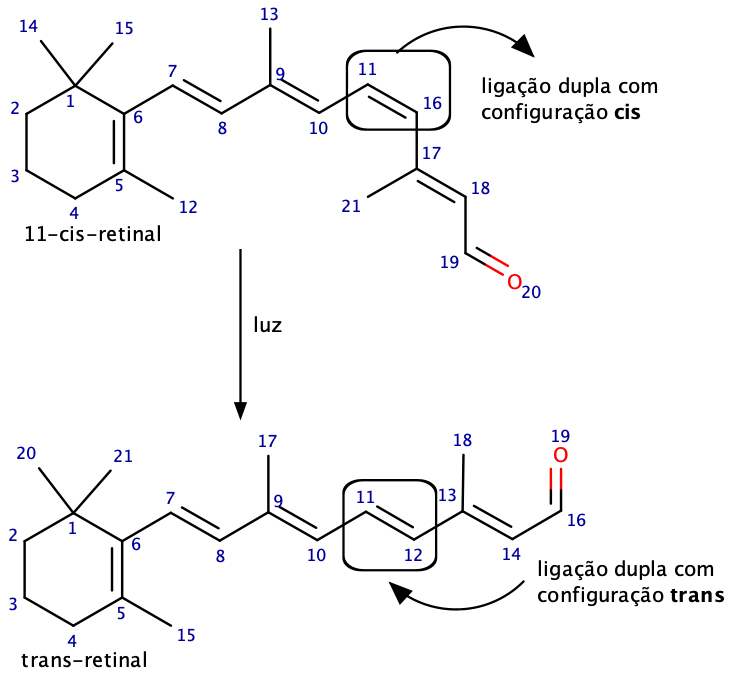
\includegraphics[width=0.7\linewidth]{imagens/cistransretinal.png}
	\caption*{Fonte: Autores}
	\label{fig:cistransretinal}
\end{figure}

Os nomes usuais dos aldeídos envolvidos no processo da visão, e mostrados na figura \ref{fig:cistransretinal} apresentam duas partes ainda não analisadas até o momento: \textbf{cis} e \textbf{trans}. São prefixos usados para citar a configuração dos substituintes de uma ligação carbono-carbono do tipo covalente dupla.

A figura \ref{fig:cistrans} ilustra dois isômeros clássicos quando se trata de isomeria cis/trans. Para melhor compreensão dos conceitos, analise a imagem e veja que existe uma linha que trespassa as duas moléculas ao longo da ligação covalente dupla. Esse será nosso eixo de referência.

Na molécula da esquerda, observamos que o átomo de carbono da esquerda da ligação dupla possui dois substituintes distintos: um átomo de Hidrogênio (destacada por um círculo ao seu redor) e um grupo metil (destacada por um quadrado so seu redor). O mesmo ocorre com o átomo de carbono da direita da ligação dupla. Repare que os dois substituintes iguais (ou semelhantes) estão \textbf{do mesmo lado do eixo de referência}: os átomos de Hidrogênio \textbf{acima} e os grupos metil \textbf{abaixo} do eixo. Assim define-se o isômero \textbf{cis}.

Na molécula da direita os grupos iguais ou semelhantes encontram-se \textbf{em lados opostos do eixo de referência} e, desta forma, define-se o isômero \textbf{trans}.		

\begin{figure}[h]
	\centering
	\caption{Exemplo de uso dos prefixos cis e trans na nomenclatura em Química Orgânica}
	\vspace{0.5cm}
	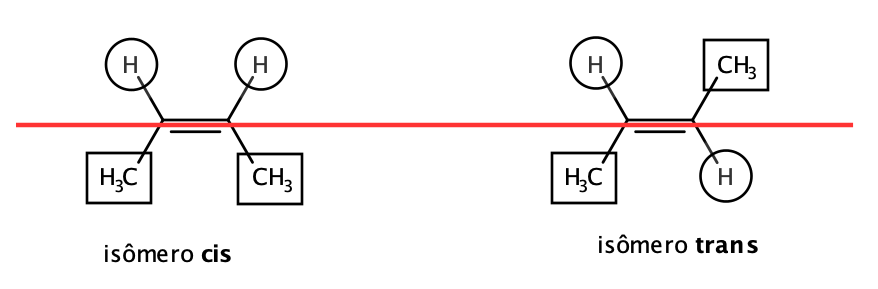
\includegraphics[width=0.85\linewidth]{imagens/cistrans.png}
	\caption*{Fonte: Autores}
	\label{fig:cistrans}
\end{figure}

Aldeídos e cetonas são duas funções orgânicas que apresentam o chamado grupo \textbf{carbonil} (C=O), o que as torna duas das mais versáteis funções da Química Orgânica. Você já ficou curioso a respeito da origem do nome da função orgânica aldeído? Espero que sim. O nome \textbf{aldeído} tem origem na expressão (em inglês) \textbf{al}cohol \textbf{dehyd}ration, comprovado pela transformação do etanol em etanal, realizada no fígado e catalisada pela enzima \textbf{álcool desidrogenase}.

O grupo carbonil é muito versátil por participar de inúmeras reações e várias delas serão discutidas nesta obra. Cabe gora uma análise estrutural do grupo carbonil, usando o mais simples dos aldeídos como exemplo.

\begin{figure}[h]
	\centering
	\caption{Estrutura do metanal}
	\vspace{0.5cm}
	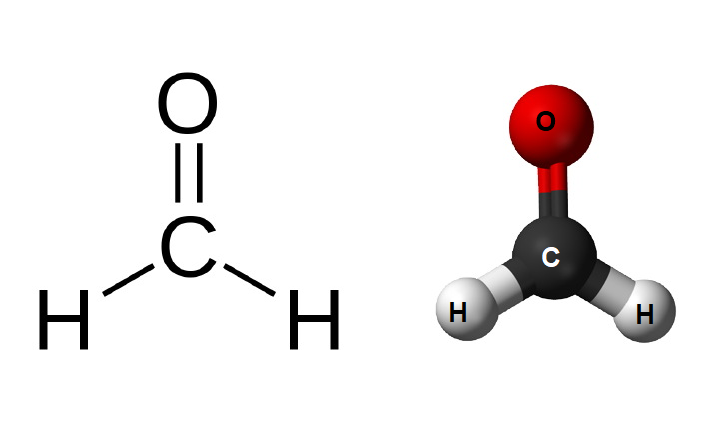
\includegraphics[width=0.35\linewidth]{imagens/formaldeido2.png}
	\caption*{Fonte: Autores}
	\label{fig:}
\end{figure}

O grupo carbonil é formado por um átomo de carbono unido a um átomo de oxigênio por uma ligação covalentes dupla, e também a dois átomos de hidrogênio por uma ligação covalente simples. 
O átomo de carbono do grupo carbono possui hibridização sp$^2$, o que confere ao grupo uma geometria plana na forma de um triângulo e agrupando as duas informações nós temos a chamada geometria \textbf{trigonal plana}, onde o ângulo diedro entre o carbono e os dois átomos de hidrogênio é de 120°. 
A planaridade do grupo carbonil permite a ocorrência de reações de adição que podem ocorrer na superfície superior ou na superfície inferior do grupo carbono, formando produtos com arranjos espaciais distintos, bastante versátil quando utilizado em reações de síntese orgânica, e, ao mesmo tempo, forma em alguns casos mistura de produtos de difícil separação.
A diferença de eletronegatividade entre o carbono e o oxigênio faz com que a ligação covalentes dupla seja polarizada e o lado negativo está mais próximo do átomo de oxigênio. Esta característica estrutural justifica a existência de híbridos de ressonância conforme pode ser visto na figura \ref{fig:hibridos} ao longo deste texto.

Usando um aldeído simples como exemplo, podemos verificar, na figura \ref{fig:etanal}, que existe uma região no grupo carbonila onde a densidade eletrônica é mais elevada, o que indica duas situações complementares entre si: 

\begin{itemize}
	\item \textbf{elevada polarização} da ligação C=O
	\item \textbf{alta reatividade} como consequência da polarização.
\end{itemize}

\begin{figure}[h]
	\centering
	\caption{Mapa de densidade eletrônica para o etanal.}
	\vspace{0.5cm}
	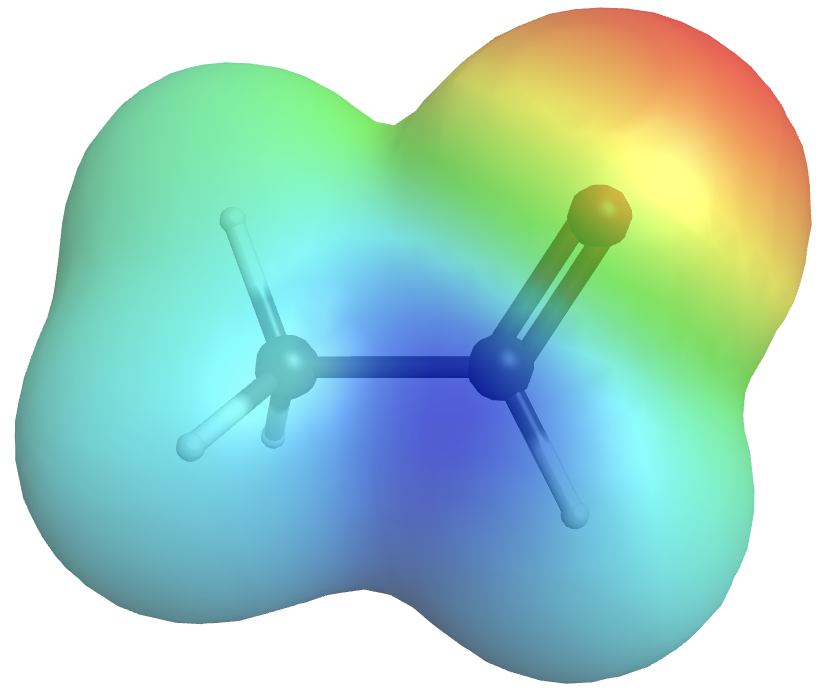
\includegraphics[width=0.5\linewidth]{imagens/etanal.png}
	\caption*{Fonte: Autores}
	\label{fig:etanal}
\end{figure}

A origem da região com elevada densidade eletrônica pode ser explicada por meio da eletronegatividade \footnote{tendência de um átomo em atrair para si os elétrons de uma ligação covalente} ou então por meio da polarizabilidade \footnote{tendência de um átomo ou molécula em ter seus elétrons deslocados por meio de um campo elétrico externo}. A diferença de eletronegatividade entre os átomos de Carbono e Oxigênio no grupo carbonila permite a existência de híbridos de ressonância, conforme mostrado na figura \ref{fig:hibridos}. Tal estrutura está envolvida nas reações orgânicas das quais os aldeídos e as cetonas participam, e que serão analisadas em outro ponto desta obra. A região com mais elevada densidade eletrônica encontra-se na parte superior esquerda da figura.

\section{Propriedades físicas}
Na ausência do híbrido de ressonância (uma vez que tais estruturas ocorrem em condições e ambientes reacionais), conforme pode ser visto na figura \ref{fig:hibridos}, com cargas elétricas positivas e negativas plenas, as moléculas de aldeídos e cetonas apresentam-se bastante polarizadas, trazendo consequências nos valores das propriedades físicas mais comuns, como Ponto de Fusão (PF), Ponto de Ebulição (PE) e Pressão de Vapor (PV). De modo geral, aldeídos e cetonas apresentam valores de PF e PE maiores que hidrocarbonetos de mesma massa molar, uma vez que suas moléculas atraem-se por meio de interações mais fortes que aquelas presentes em hidrocarbonetos. Veja a tabela \ref{pfalcanos} para alguns valores que comprovam nossa breve análise.

\vspace{0.5cm}
\begin{table}[!h]
	%\begin{tabular}
	\begin{center}
	\caption{\label{pfalcanos}Comparativo de propriedades físicas (PE, em $^o$C) de hidrocarbonetos, aldeídos e cetonas (a menos cetona possível possui 3 carbonos em sua estrutura).}
	\vspace{0.5cm}
	\begin{tabular}{c c c c}
	\hline
	Num. carbonos & Alcano & Aldeído & Cetona\\
	\hline
	1 & -162 & -19,5 & -- \\
	2 & -89 & 20,2 & -- \\
	3 & -42 & 48.8 & 56,2 \\
	4 & 0 & 74,8 & 79,6 \\
	5 & 36 & 100,3 & 101 \\
	\hline
	\end{tabular}
	\end{center}
	\caption*{Fonte: Autores}
\end{table}

\begin{figure}[h]
	\centering
	\caption{Híbridos de ressonância no etanal}
	\vspace{0.5cm}
	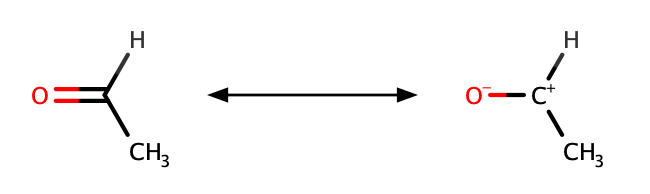
\includegraphics[width=0.85\linewidth]{imagens/hibridos.png}
	\caption*{Fonte: Autores}
	\label{fig:hibridos}
\end{figure}

A polaridade de uma molécula (polar ou apolar) pode ser determinada, de modo muito simples, ao dissolve-la em um solvente polar ou apolar. Sabendo que moléculas polares dissolvem-se em solventes polares e que ocorre o mesmo para moléculas apolares, um teste químico em laboratório pode concluir se a molécula é polar ou não.

Porém, pode ser necessário saber o quão polar ou apolar é essa molécula, e esta tarefa pode ser feita com ajuda de um software aplicado à Química Orgânica, como por exemplo \cite{avogadro}, utilizado na construção de algumas imagens nesta obra. A figura \ref{fig:polaridade} mostra o resultado do cálculo da polaridade do etanal. 

\begin{figure}[h]
	\centering
	\caption{Polaridade calculada do etanal}
	\vspace{0.5cm}
	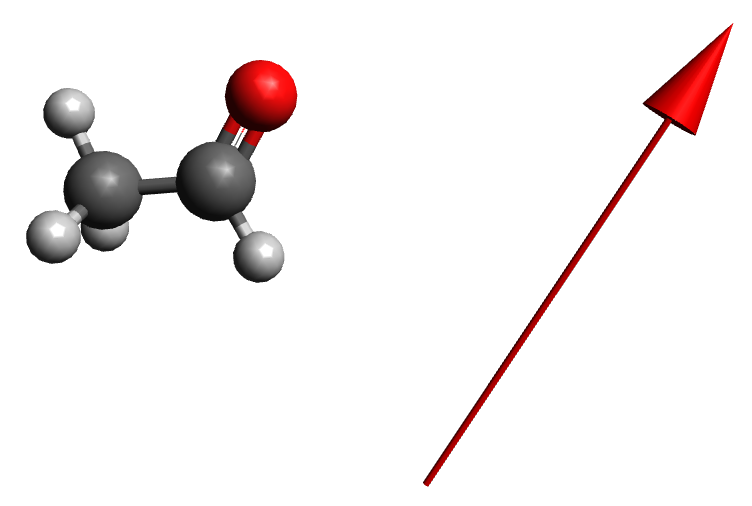
\includegraphics[width=0.75\linewidth]{imagens/polaridadeetanal}
	\caption*{Fonte: Autores}
	\label{fig:polaridade}
\end{figure}

Embora pareça desproporcional, a seta à direita da imagem \ref{fig:polaridade} é desenhada pelo software após o cálculo do momento dipolar do etanal \cite{raymond2015chemistry}. O calor calculado é de \textbf{2,472 D} (Debye). Apenas como referência, a água é conhecida por ser um solvente polar, apresenta momento dipolar de \textbf{1,855 D}, mostrando que o etanal é bem mais polar que a água, ou seja, apresenta assimetria na distribuição de cargas elétricas muito maior que na água \footnote{Momento dipolar é uma grandeza vetorial que representa a polaridade de um sistema de cargas elétricas. É definido como o produto da carga elétrica pela distância entre as cargas, e tem a direção do segmento de reta que une os centros das cargas, apontando ao lado maior densidade eletrônica.}.

Essa polaridade elevada faz com que o etanal seja solúvel em água para quaisquer proporções, assim como o etanol, e uma simulação realizada com o software Avogadro \cite{avogadro} mostrou a formação de uma ligação de Hidrogênio entre o átomo de Oxigênio do grupo carbonil e um dos átomos de Hidrogênio da água. Uma imagem dessa simulação pode ser vista na figura \ref{fig:etanalagua}, onde o tracejado representa a ligação de Hidrogênio. Na figura, por uma característica do software, os átomos de Hidrogênio são as bolinhas claras e menores, os átomos de Carbono são as bolinhas maiores e mais escuras, enquanto os átomos de Oxigênio são as bolinhas de tamanho intermediário e de cor vermelha.

Naturalmente, estas ligações de Hidrogênio não ocorrem apenas com um dos átomos de Hidrogênio da água, mas sim \textbf{todos} os átomos de Hidrogênio da água e com os dois pares eletrônicos não compartilhados do átomo de Oxigênio, formando uma espécie rede intermolecular, parecida com a que ocorre entre moléculas de água. Tal fato ajuda a explicar a elevada solubilidade do etanal em água.
 
\begin{figure}[H]
	\centering
	\vspace{0.25cm}
	\caption{Formação de ligação de hidrogênio entre etanal e água.}
	\vspace{0.25cm}
	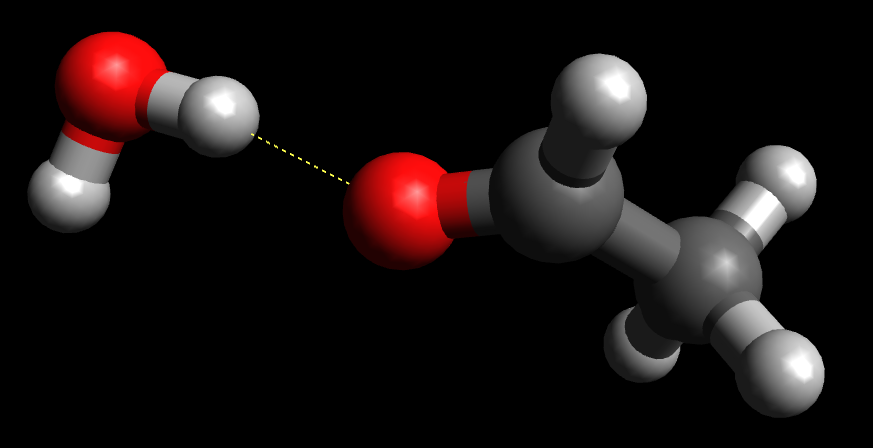
\includegraphics[width=0.85\linewidth]{imagens/etanal_agua.png}
	\caption*{Fonte: Autores}
	\label{fig:etanalagua}
\end{figure}

E os demais aldeídos? Apresentam o mesmo comportamento? Não, não apresentam. Aldeídos com cadeias carbônicas maiores sofrem mais a influência da baixa polaridade da porção hidrocarboneto, comparada com o grupo carbonil, e são menos solúveis em água.

Cetonas apresentam o mesmo comportamento dos aldeídos quando se trata de solubilidade em água, e cetonas com moléculas pequenas são bem solúveis em água, e, à medida em que as cadeias carbônicas aumentam de tamanho, ajudam a quebrar as eventuais ligações de Hidrogênio entre aldeídos ou cetonas e água. Isso explica a diminuição da solubilidade, em água, de aldeídos e cetonas com cadeias carbônicas maiores.

\section{Nomenclatura}
A nomenclatura de aldeídos e cetonas está diretamente relacionada com a presença do grupo carbonil, e apresentam diferentes sufixos:
 \begin{itemize}
	\item \textbf{aldeídos}: al
	\item \textbf{cetonas}: ona
 \end{itemize}

 \subsection{Aldeídos}
A principal característica estrutural de aldeídos é o grupo funcional localizar-se sempre na extremidade do hidreto pai. Com isso, a numeração da cadeia para identificação precisa dos localizadores inicia-se sempre na posição do grupo funcional.

\begin{figure}[h]
	\centering
	\vspace{0.25cm}
	\caption{Exemplo de nomenclatura de aldeído acíclico.}
	\vspace{0.25cm}
	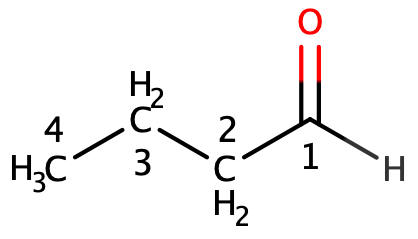
\includegraphics[width=0.45\linewidth]{imagens/butanal.png}
	\caption*{Fonte: Autores}
	\label{fig:butanal}
\end{figure}

A composição do nome do aldeído é realizada utilizando-se a nomenclatura substitutiva, onde o sufixo \textbf{o} do hidreto pai é substituído pelo sufixo \textbf{al} dos aldeídos. Um hidrocarboneto com quatro carbonos chama-se \textbf{butano} e, portanto, o aldeído com mesmo número de átomos de carbono, exibido na figura \ref{fig:butanal}, chama-se \textbf{butanal}.

Quando o aldeído é substituído, ou seja, um ou mais átomos de Hidrogênio foram substituídos por outros átomos ou grupos de átomos, todos os substituintes precisam ter seu nome e localização na cadeia carbônica, seguindo a ordem alfabética dos nomes dos substitutintes, conforme pode ser visto na figura \ref{fig:aldeidosubst}.

\begin{figure}[H]
	\centering
	\vspace{0.25cm}
	\caption{Exemplo de nomenclatura de aldeído acíclico e substituído.}
	\vspace{0.25cm}
	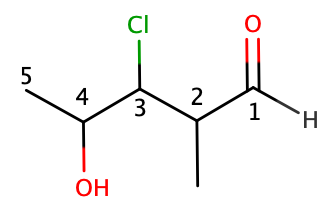
\includegraphics[width=0.45\linewidth]{imagens/aldeidosubst.png}
	\caption*{Fonte: Autores}
	\label{fig:aldeidosubst}
\end{figure}

O aldeído ilustrado na figura \ref{fig:aldeidosubst} apresenta três substituintes e, portanto, precisamos definir três localizadores. Considerando os nomes dos substitutintes (metil, cloro e hidroxi), a ordem alfabética destes é \textbf{cloro}, \textbf{hidroxi} e \textbf{metil}. Para compor o nome do aldeído, cite os nomes dos substituintes em ordem alfabética, mas explicitando os respectivos localizadores (3, 4 e 2). Assim, o nome do aldeído é \textbf{3-cloro-4-hidroxi-2-metil-pentanal}.

O cenário muda ligeiramente quando o hidreto pai do aldeído apresenta cadeia cíclica. Nestes casos, o sufixo do aldeído passa a ser \textbf{carbaldeído} e o átomo de Carbono que sustenta o grupo funcional é numerado como 1, com ao menos uma exceção, discutida a seguir, relacionada ao hidrocarboneto chamado \textbf{naftaleno}, ilustrado na figura \ref{fig:naftaleno}.

\begin{figure}[h]
	\centering
	\vspace{0.5cm}
	\caption{Naftaleno}
	%\vspace{0.25cm}
	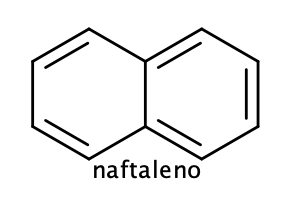
\includegraphics[width=0.25\linewidth]{imagens/naftaleno.png}
	\caption*{Fonte: Autores}
	\label{fig:naftaleno}
\end{figure}

Esta molécula é bastante simétrica e, portanto, não existem tantas posições distintas na cadeia cíclica como se pode perceber ao analisar a imagem rapidamente. Precisamos lembrar, neste momento, de um conceito simples: \textbf{plano de simetria}. Esta entidade pode ser compreendida como um corte que pode ser feito em, por exemplo, algum objeto e que o divide em duas metades idênticas. 

A molécula do naftaleno admite \textbf{dois planos de simetria}, um deles ao longo da ligaçào covalente comum aos dois ciclos e outro perpendicular a esse primeiro, que dividem a molécula em \textbf{quatro partes idênticas}. Considere qua o naftaleno possui fórmula molecular \ce{C10H8} e estes 8 átomos de Hidrogênio serão igualmente divididos em cada uma dessas quatro partes idênticas. Assim, temos apenas \textbf{dois átomos de Hidrogênio distintos} e não 8 como se percebe sem analisar os conceitos de simetria.

A análise cuidadosa da imagem \ref{fig:simetria} mostra os três planos de simetria presentes na molécula de naftaleno (incluindo aquele que trespassa os átomos ao meio), dividindo-a em quatro quadrantes idênticos, cada um deles contendo dois átomos de Carbono e dois átomos de Hidrogênio. Repare que todos os átomos de carbono estão todos no mesmo plano na posição central da imagem e identificados por meio de bolinhas escuras, conectadas entre si.

\begin{figure}[h]
	\centering
	\vspace{0.5cm}
	\caption{Elementos de simetria presentes no naftaleno}
	%\vspace{0.25cm}
	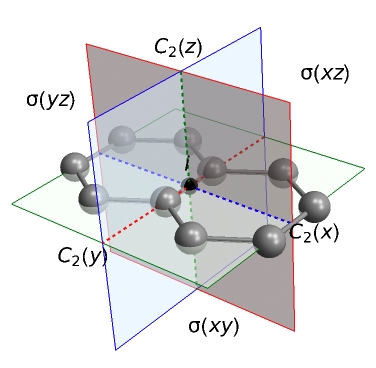
\includegraphics[width=0.5\linewidth]{imagens/simetria.png}
	\caption*{Fonte: Verifique nas referências}
	\label{fig:simetria}
\end{figure}

Uma outra imagem pode deixar o conceito todo ainda mais claro \cite{sym13040526}, como pode ser observado na figura \ref{fig:simetria2}.

\begin{figure}[h]
	\centering
	\vspace{0.5cm}
	\caption{Simplificação dos elementos de simetria presentes no naftaleno}
	%\vspace{0.25cm}
	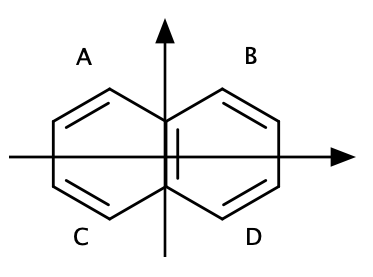
\includegraphics[width=0.35\linewidth]{imagens/simetria3.png}
	\caption*{Fonte: Autores}
	\label{fig:simetria2}
\end{figure}

Na figura \ref{fig:simetria2}, podemos perceber que a combinação das duas setas divide a molécula do naftaleno em quatro quadrantes \textbf{idênticos}, identificados pelas letras A, B, C e D. Atente-se ao fato de que os quadrantes A e B são \textbf{imagens especulares} um do outro e que ocorre o mesmo entre os quadrantes C e D. Ainda, os quadrantes A e C também são imagens especulares um do outro, assim como os quadrantes B e D. Os dois átomos de Carbono e os dois átomos de Hidrogênio em cada quadrante são diferentes entre si, o que justifica a numeração oficial do naftaleno, vista na figura \ref{fig:numerado}. Tecnicamente, um \textbf{eixo de simetria} é diferente de um \textbf{plano de simetria}, mas a simetria do naftaleno não mudou com a representação simplificada, e o uso das setas pode deixar o tópico mais claro para alguns leitores.

\begin{figure}[h]
	\centering
	\vspace{0.5cm}
	\caption{Numeração oficial do naftaleno}
	%\vspace{0.25cm}
	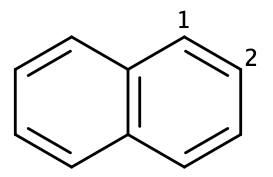
\includegraphics[width=0.35\linewidth]{imagens/numerado.png}
	\caption*{Fonte: Autores}
	\label{fig:numerado}
\end{figure}

Compreendida a numeração da cadeia carbônica do naftaleno, podemos analisar a segunda parte de nossa exceção, para que o nome de um aldeído visto pouco adiante fique plenamente esclarecida.

Repare que a molécula do naftaleno (figura \ref{fig:naftaleno}) apresenta cinco ligações covalentes duplas e, para "desaromatizar" o naftaleno por um processo chamado de \textbf{hidrogenação} (reação orgânica que consiste na adição de moléculas de H$_2$ a cadeias insaturadas, na proporção de \textbf{1 molécula de H$_2$ para cada ligação dupla}), são necessárias 5 moléculas de H$_2$ ou 10 átomos de Hidrogênio, conforme pode ser visto na figura \ref{fig:hidrogenacao}. Não foram citadas na reação a presença de qualquer catalisador e tampouco condições de temperatura e pressão, uma vez que trata-se de um esquema simplificado. Em tempo: a molécula formada através da hidrogenação do naftaleno (deca-hidronaftaleno) mantém a mesma numeração do naftaleno.

\begin{figure}[h]
	\centering
	\vspace{0.5cm}
	\caption{Reação de hidrogenação do naftaleno}
	%\vspace{0.25cm}
	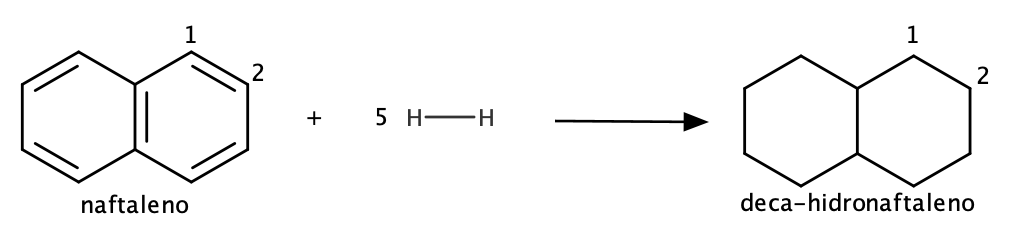
\includegraphics[width=1\linewidth]{imagens/hidrogenacao.png}
	\caption*{Fonte: Autores}
	\label{fig:hidrogenacao}
\end{figure}

Podemos analisar agora um conjunto de moléculas da função aldeído, visto na figura \ref{fig:conjunto}, inicialmente identificados pelas letras A, B, C e D, onde praticaremos as regras de nomenclatura de aldeídos, herdando as regras gerais da IUPAC. Lembre-se que é necessário identificar o hidreto pai, bém os localizadores, pois cada substituinte exige seu localizador correspondente e, no caso de mais de um substituinte, considere sempre ordem alfabética ao citar os mesmos.

\begin{figure}[H]
	\centering
	\vspace{0.5cm}
	\caption{Exemplos de nomes de aldeídos diversos}
	%\vspace{0.25cm}
	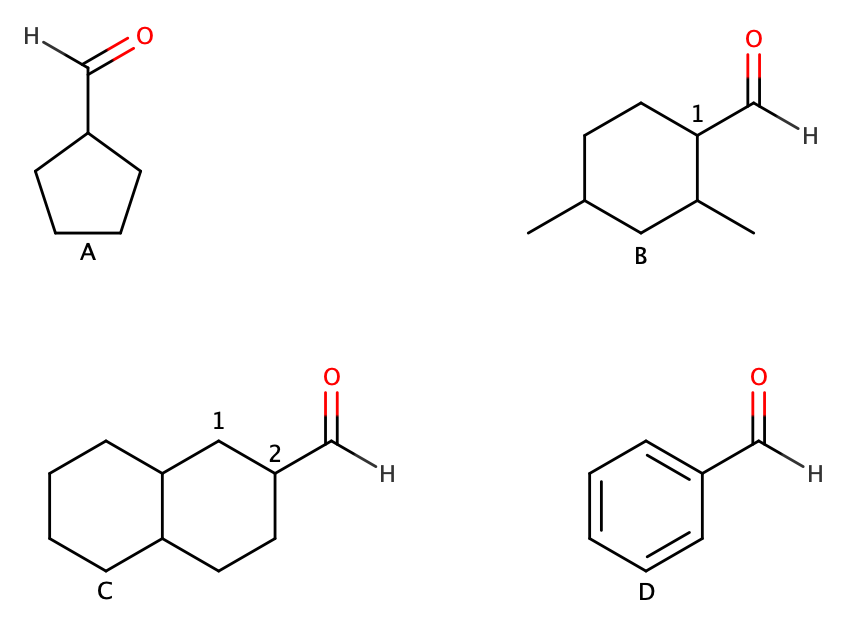
\includegraphics[width=0.65\linewidth]{imagens/exemplosaldeidos.png}
	\caption*{Fonte: Autores}
	\label{fig:conjunto}
\end{figure}

\begin{description}
	\item[\textbf{Substância A}]: trata-se de um aldeído no qual o hidreto pai é uma cadeia cíclica e, portanto, o grupo carbonil passa a chamar-se \textbf{carbaldeído} e ligado à posição do anel ciclopentânico. Assim, o nome da substância é \textbf{ciclopentanocarbaldeído}. 
	\item[\textbf{Substância B}]: o hidreto pai deste aldeído é o hidrocarboneto chamado ciclo-hexano e o grupo carbonil está ligado ao carbono numerado como 1 na cadeia do hidreto pai. Existem ainda dois substitutintes chamados \textbf{metil} com os localizadores 2 e 4. Assim, este aldeído é chamado de \textbf{2,4-dimetil-ciclo-hexanocarbaldeído}. 
	\item[\textbf{Substância C}]: este aldeído é derivado do naftaleno por meio da reação de hidrogenação total. Repare que o hidreto pai, conforme visto anteriormente, chama-se \textbf{deca-hidronaftaleno}, porque a reação de hidrogenação inseriu 10 novos hidrogênios, o que justifica o prefixo \textbf{deca}. O grupo funcional encontra-se na posição 2 do hidreto pai, conforme discutido anteriormente. Portanto, o nome do aldeído aqui analisado é \textbf{deca-hidronafataleno-2-carbaldeído}.  
	\item[\textbf{Substância D}]: o nome desta substância é mais simples que os demais, uma vez que o substituinte formado por um átomo de Carbono ligado ao anel aromático é chamado de \textbf{benzil}, considerado legado pela IUPAC. Portanto, o nome deste aldeído é \textbf{benzaldeído}.
\end{description}

 \subsection{Cetonas}
 
 \begin{minipage}{\textwidth} 
 	\begin{figure}[H]
 		\caption{\label{fig:label} Figure title}
 		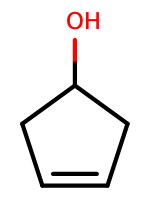
\includegraphics[width=0.25\linewidth]{imagens/cpd.png}
 	\end{figure}
 \end{minipage}
